\documentclass{report}

\usepackage[ngerman]{babel}
\usepackage[utf8]{inputenc}
\usepackage[T1]{fontenc}
\usepackage{hyperref}
\usepackage{csquotes}
\usepackage[a4paper]{geometry}
\usepackage{graphicx}

\usepackage[
    backend=biber,
    style=apa,
    sortlocale=de_DE,
    natbib=true,
    url=false,
    doi=false,
    sortcites=true,
    sorting=nyt,
    isbn=false,
    hyperref=true,
    backref=false,
    giveninits=false,
    eprint=false]{biblatex}
\addbibresource{../references/bibliography.bib}


\title{Ethik im Umgang mit Daten} 
\author{Ruben Nussbaumer}
\date{\today}


\begin{document}

\maketitle

\abstract{
    In diesem Dokument zeige ich auf, wie KI funktioniert und was KI überhaupt ist. 
    Danach erkläre ich und zeige ich auf, wie KI im Zusammenhang mit Ethik steht und habe noch einige Fragen zu diesem Thema beantwortet, wie z.B. bei welchen Sachen KI ein Ethisches Gewissen braucht usw.
}

\tableofcontents

\chapter{Einleitung}
Haben Sie sich schon einmal gefragt, wie KI funktioniert und ob KI auch eine Art Persöhnlichkeit haben kann und somit auch Entscheidungen treffen, die normalerweise Gefühle brauchen.
Ob und wie KI mit Ethischen Entscheidungen funktioniert und welche positiven und negativen Auswirkungen das haben kann, beantworte ich in diesem Paper.
Da das selber meine erste Auseinandersetzung mit KI und Ethik ist, habe ich selbst sehr viel gelernt, bei dieser Arbeit.
Diese Arbeit dient dazu, dass man sich einen Überblick machen über dieses Thema machen kann und danach kann man sich selbst vertiefen, wenn man möchte.
\section{Was ist eine KI?}
Künstliche Intelligenz (KI) ist ein Teilgebiet der Informatik. Sie imitiert menschliche kognitive Fähigkeiten, indem sie Informationen aus Eingabedaten erkennt und sortiert. Diese Intelligenz kann auf programmierten Abläufen basieren oder durch maschinelles Lernen erzeugt werden

\section{Wie funktioniert KI?}
KI beinhaltet eine grosse Zahl an Technologien, die das Ziel hat Maschinen und Computern die Fähigkeit
zu geben, Aufgaben, welche Menschen Zeit braucht, selbstständig zu erledigen, was normalerweise eine Menschliche Intelligenz benötigt.
Die Grundlegenden Konzepte, wie KI mit diesen Technologien beschaffen ist, sind in den folgenden Abschnitten beschrieben.
\subsection{Daten}
Die Grundlagen, die KI braucht um überhaupt zu funktionieren, sind Daten. KI bezieht ihr Wissen und die Infos, die sie braucht aus Daten, 
die ihr eingeschleust wurden.
\subsection{Maschinelles Lernen}
KI lernt viel durch Maschinelles Lernen. Sie haben sicher schon einmal gesehen, wie eine KI in einem Spiel platziert wird und diese solange
das Spiel zu verstehen lernt, bis es das ganze Spiel spielen kann. z.B. bei Super Mario.

\subsection{Neuronale Netzwerke}
Neuronale Netzwereke sind eine der bekanntsten Art von KI. Neuronale Netzwerke basieren auf der Funktionsweise vom menschlichen Gehirn. Die Netzwerke bestehen aus ganz vielen verbundenen Konten (Neuronen), welche in sogenannten Schichten organisisiert werden. 
Es gibt die Eingabeschicht, verborgene Schichten und die Ausgabeschicht. Jedes Neuron erhält Signale und bearbeitet diese durch gewichtete Verbindungen und leitet ein Signal weiter. Diese Gewichte werden während des Trainings angepasst, damit das Netzwerk noch genauer funktioniert.
 Mit Aktivierungsformen kann man mit Neuronalen Netzwerken Bzeihungen in den Daten erstellen, also Zusammenhänge zwischen Daten erkennen lassen. Tiefe neuronale Netzwerke mit ganz vielen Schichten werden als deep learning bezeichnet und erkennen sehr Komplexe Zusammenhänge. 
 Das verwendet man z.B bei Bilderkennung. Wenn ein Netzwerk trainiert ist, kann man es benutzen um Vorhersagen usw. zu treffen mit neuen Daten.

\subsection{Deep Learning}
Deep learning ist eine fortgeschrittene Methode des Maschinellen Lernens, welche tiefe neuronale Netzwerke verwendet, um umfangreiche Muster in sehr grossen Datenmengen zu erkennen. Die neuronalen Netzwerke haben viele Schichten von Neuronen, welche Automatisch dazu lernen, was wichtig ist und man braucht keinen Menschen dazu. Deep Learning benutzt man mit Neuronalen Netzwerken um Bilderkennnung und Spracherkennung usw. zu betreiben.
\subsection{Anwendungen der KI}
\begin{itemize}
    \item KI kann dabei helfen, die Fehlereffekte zu reduzieren.
    \item Spracherkennung
    \item Bildverarbeitung
    \item Automatisierung
    \item Empfehlungen auf persöhnlichen Interessen basierend
    \item Spieleintelligenz
\end{itemize}
\begin{figure}[h]

    \centering 
 
    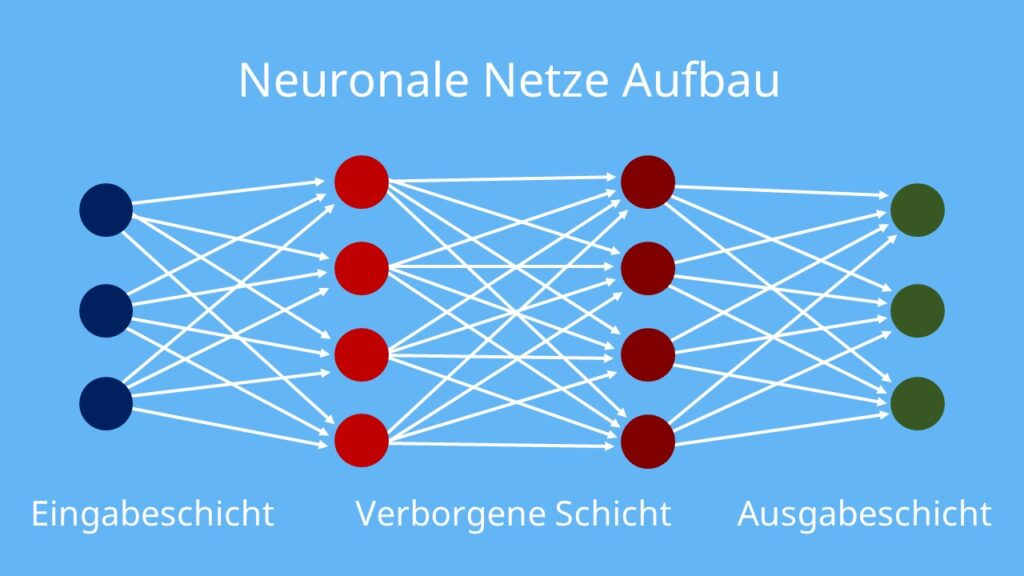
\includegraphics[width=0.65\textwidth]{img.jpg} 
 
    \caption{Neurale-Netzwerk-Grafik, Studyflix}
 
    \label{fig:meme}
 
 \end{figure}
 

\chapter{KI und Ethik}
KI und Ethik sind eigentlich zwei Begriffe, welche man meist nicht in einen gemeinsamen Zusammenhang bringt. Dennoch stehen sie sehr nahe zueinander und es ist sehr wichtig dass KI etwas von Ethik versteht und  wir auch wissen in welchem Zusammenhang wir KI Ethik beibringen sollen.
In diesem Kapitel erkläre ich, was Ethik überhaupt ist,was KI und Ethik überhaupt miteinander zutun haben, wie KI ethisch helfen kann, wie sie schaden kann usw.
Es ist wichtig, dass wir uns bewusst sind, wie wir KI trainieren und auch  wissen zu was KI alles fähig ist heutzutage.
\section{Was ist Ethik?}
Ethik ist ein Teilgebiet der Philosophie, welcher sich mit den Fragen befasst, ob etwas moralisch richtig oder falsch ist und welche Prinzipien, Werte und Konzepte unsere Handlungen und Entscheidungen leiten sollte. 
Wie z.B. ob es richtig ist jemanden zu töten, der selbst eine Person getötet hat.
Meiner Meinung kann, was ethisch korrekt ist sehr subjektiv sein, wie bei dem oben genannten Problem zum Beispiel. Daher gibt die Gesellschaft ein bisschen ab, was ethisch korrekt ist und was nicht. 
Sachen wie z.B. die Natur kaputt zu machen sind generell als ethisch unkorrekt bezeichnet.
\section{Wie kann Ki ethisch helfen?}
\begin{itemize}
    \item Verbesserung der Entscheidungsfindung: Dadurch, dass KI grosse Datenmengen aufs mal verarbeiten kann, kann sie dabei helfen sehr grosse und komplexe Entscheidungen zu optimieren und Positive, so wie negative Askepte aufzuzählen. 
    \item Förderung der Gerechtigkeit: Es kann von KI geholfen werden, Vorurteile und Diskriminierung zu identifizieren und zu bekämpfen. Es können Algorithmen verwendet werden umd unfaire Sachen im Rechtswesen aufzuzeigen und zu verbessern.
    \item Unterstützung der Nachhaltigkeit: Es können Lösungen für Ökologische Probleme entwickelt werden, wie z.B die Verbesserung des Energieverbrauchs, dem Erhalt von Wasser oder der Erfindung von Landwirtschaftlichen Methoden.
    \item Medizin: Diagnosen können verbessert werden, Behandlungsgespräche können von KI gehalten werden um Ärzte zu entlasten und Ideen entwickeln um Medizinische Versorgung zugänglicher zu machen.
    \item Bildung: Bildungsressourcen können personalisiert werden und erweitert werden, sodass mehr Menschen Zugang zu Bildung haben.
    \item Forschung: KI kann kann helfen, neue Sachen herauszufinden oder Prozesse wöhrend der Forschung zu beschleunigen und zu erleichtern, wie z.B. Analyse von Proben.
\end{itemize}

\section{Wie kann Ki ethisch schaden?}
\begin{itemize}
    \item Missinformation: Man weiss nie ob das was KI sagt richtig oder falsch ist, dadurch können Informationen gegeben werden von KI, welche nicht stimmen und das kann zu etwas unethischem führen wie ein Gesetzesbruch z.B.
    \item Sicherheitsrisiken: KI kann bei sicherheitskritischen Sachen, wie zum Beispiel automatisches Fahren eingesetzt werden und wenn es dort fehler gibt kann es grosse Schäden verursachen.
    \item Verletzung der Privatsphäre: Wenn man einer KI nicht richtig beibringt mit Daten von Menschen umzugehen, kann die AI vielleicht persönliche Daten weitergeben, oder diese Infos irgendwie schädlich verwenden.
    \item Verlust von Arbeitsplätzen: Dadurch, dass KI vieles automatisiert braucht man viele Jobs vielleicht bald nicht mehr, da diese von KI erledigt werden können und so verlieren viele Menschen ihre Arbeit und es würde sich auf die Wirtschaft auswirken, in dem die Reichen reicher werden und die Armen ärmer.
    \item Krieg: KI kann im Krieg eingesetzt werden und dann ausspionieren, angreifen usw. Da ich Krieg moralisch nicht vertretbar finde its es auch nicht gut KI im Krieg eizusetzen.
\end{itemize}

\section{Wie verhindert man unethische Taten der KI?}
\begin{itemize}
    \item Ethische Grundsätze und Leitlinien beibringen und klarstellen in der Entwicklung der KI. Hängt natürlich davon ab wer schreibt und was er als ethisch empfindet.
    \item Regulierung und Gesetzgebung: Man sollte gesetze erlassen die den ethischen Einsatz von KI sicherstellt. Man sollte auch International zusammenarbeiten um einheitliche Standarts zu schaffen.
    \item Technische Massnahmen: Man sollte mit deep learning der KI beibringen, was Ethisch korrekt ist und was nicht und das auch International anwenden.
    \item Regulierung der Benutzung: Nicht jeder sollte KI benutzen können, damit nicht unbedingt böse Menschen die KI nutzen. Eine Lizenz vielleicht? 
\end{itemize}

\section{Fazit und persönliche Meinung}
Also ich finde KI kann sehr nützlich sein für mich. In der Schule z.B. hilft es mir sehr KI zu benutze, aber es gibt auch Sachen, bei denen ich KI noch gar nicht gut finde, wie z.B. bei Codeium.
KI kann sehr schlecht sein, aber auch sehr gut und für gute Zwecke verwendet werden, wie wir gesehen haben in den oberen Abschnitten. 
Meiner Meinung nach könnte man die unethische Nutzung von KI regeln, durch verschiedene Arten von KI, welche verschiedene Bereiche abdecken und für die jeweiligen Bereiche, um diese zu benutzen eine Lizenz und Berechtigung zu verlangen.
 Dadurch könnte man ein bisschen einschränken, wer KI nutzen kann, welche wirklich schädlich sein kann ethisch gesehen.
\printbibliography

\end{document}
